%
%===============>>  ГРУППА 11-1 МОДУЛЬ 7  <<=============
%
\setmodule{7}

%BEGIN_FOLD % ====>>_____ Занятие 1 _____<<====
\begin{class}[number=1]
	\begin{listofex}
		\item %484557
		\begin{tasks}(1)
			\task Решите уравнение \( (2\sin x+\sqrt{3}) \cdot \sqrt{\cos x}=0 \)
			\task Найдите все корни этого уравнения, принадлежащие отрезку: \( \left[ \dfrac{3\pi}{2}; \dfrac{7\pi}{2} \right] \)
		\end{tasks}
		\item %505102
		\begin{tasks}(1)
			\task Решите уравнение \( 9^{\sin{x}}+9^{-\sin x}=\dfrac{10}{3} \)
			\task Найдите все корни этого уравнения, принадлежащие отрезку: \( \left[ -\dfrac{7\pi}{2}; -2\pi \right]  \)
		\end{tasks}
		\item %505236
		\begin{tasks}(1)
			\task Решите уравнение \( \left( \dfrac{2}{5} \right)^{\cos x}+ \left( \dfrac{5}{2} \right)^{\cos x}=2 \)
			\task Найдите все корни этого уравнения, принадлежащие отрезку: \( \left[ -3\pi;-\dfrac{3\pi}{2} \right]  \)
		\end{tasks}
		\item %501689
		\begin{tasks}(1)
			\task Решите уравнение \( 15^{\cos x}=3^{\cos x} \cdot 5^{\sin x} \)
			\task Найдите все корни этого уравнения, принадлежащие отрезку: \( \left[ 5\pi; \dfrac{13\pi}{2} \right]  \)
		\end{tasks}
		\item %505565
		\begin{tasks}(1)
			\task Решите уравнение \( \dfrac{3^{\cos x}}{9^{\cos^2x}}=4^{2\cos^2x-\cos x} \)
			\task Найдите все корни этого уравнения, принадлежащие отрезку: \( \left[ -\dfrac{3\pi}{2}; \dfrac{\pi}{6} \right]  \)
		\end{tasks}
		\item %501729
		\begin{tasks}(1)
			\task Решите уравнение \( (27^{\cos x})^{\sin x}=3^{\frac{3\cos x}{2}} \)
			\task Найдите все корни этого уравнения, принадлежащие отрезку: \( \left[ -\pi; \dfrac{\pi}{2} \right]  \)
		\end{tasks}
		
		\item %500192
		\begin{tasks}(1)
			\task Решите уравнение \( \left( \dfrac{1}{81} \right)^{\cos x}=9^{2\sin{2x}} \)
			\task Найдите все корни этого уравнения, принадлежащие отрезку: \( [-3\pi; -2\pi] \)
		\end{tasks}
	\end{listofex}
\end{class}
%END_FOLD

%BEGIN_FOLD % ====>>_____ Занятие 2 _____<<====
\begin{class}[number=2]
	\begin{listofex}
		\item %501483
		\begin{tasks}(1)
			\task Решите уравнение: \( 36^{\sin 2x} = 6^{2\sin x} \)
			\task Найдите все корни этого уравнения, принадлежащие отрезку: \( \left[ -\dfrac{7\pi}{2}; - \dfrac{5\pi}{2} \right]  \)
		\end{tasks}
		\item %508390
		\begin{tasks}(1)
			\task Решите уравнение: \( 5^{2\sin2x}= \left( \dfrac{1}{25} \right)^{\cos{(\frac{3\pi}{2}+x)}}  \)
			\task Найдите все корни этого уравнения, принадлежащие отрезку: \( \left[ \dfrac{3\pi}{2}; 3\pi \right] \)
		\end{tasks}
		\item %514650
		\begin{tasks}(1)
			\task Решите уравнение: \( 2^{4\cos x} + 3 \cdot 2^{2\cos x} -10 = 0 \)
			\task Найдите все корни этого уравнения, принадлежащие отрезку: \( \left[ \pi; \dfrac{5\pi}{2} \right] \)
		\end{tasks}
		\item %516331
		\begin{tasks}(1)
			\task Решите уравнение: \( \dfrac{2\sin^2{x} - \sin x}{\log_7 (\cos x)} = 0 \)
			\task Найдите все корни этого уравнения, принадлежащие отрезку: \( \left[ -5\pi; -\dfrac{7\pi}{2} \right] \)
		\end{tasks}
		\item %516274
		\begin{tasks}(1)
			\task Решите уравнение: \( \dfrac{9^{\sin 2x} - 3^{2\sqrt{2} \sin x}}{\sqrt{11 \sin x}} = 0 \)
			\task Найдите все корни этого уравнения, принадлежащие отрезку: \( \left[ \dfrac{7\pi}{2}; 5\pi \right] \)
		\end{tasks}
		\item %515648
		\begin{tasks}(1)
			\task Решите уравнение: \( \dfrac{(\tg x + \sqrt{3}) \log_{13} (2\sin^2{x}) }{\log_{31} (\sqrt{2}\cos x)}=0 \)
			\task Найдите все корни этого уравнения, принадлежащие отрезку: \( \left[ \dfrac{3\pi}{2}; \dfrac{5\pi}{2} \right] \)
		\end{tasks}
	\end{listofex}
\end{class}
%END_FOLD

%BEGIN_FOLD % ====>>_ Домашняя работа 1 _<<====
\begin{homework}[number=1]
	\begin{listofex}
		\item %525117
		\begin{tasks}(1)
			\task Решите уравнение: \( 2\log_2^2 (2\cos x) - 9 \log_2 (2\cos x) +4 = 0 \)
			\task Найдите все корни этого уравнения, принадлежащие отрезку: \( \left[ -2\pi; -\dfrac{\pi}{2} \right] \)
		\end{tasks}
		\item %500447
		\begin{tasks}(1)
			\task Решите уравнение: \( \log_2 (\cos x + \sin{2x} + 8) = 3 \)
			\task Найдите все корни этого уравнения, принадлежащие отрезку: \( \left[ \dfrac{3\pi}{2}; 3\pi \right] \)
		\end{tasks}
		\item %517438
		\begin{tasks}(1) 
			\task Решите уравнение: \( 8 \cdot 16^{\cos x} - 6 \cdot 4^{\cos x} + 1 = 0 \)
			\task Найдите все корни этого уравнения, принадлежащие отрезку: \( \left[ \dfrac{3\pi}{2}; 3 \pi \right] \)
		\end{tasks}
		\item %
		\begin{tasks}(1)
			\task Решите уравнение: \( 16^{\sin (\pi+x)}= \left( \dfrac{1}{2} \right)^{4\sin{(\frac{5\pi}{2}+x)}} \)
			\task Найдите все корни этого уравнения, принадлежащие отрезку: \( \left[ \dfrac{3\pi}{2}; 3\pi \right] \)
		\end{tasks}
		\item %523994
		\begin{tasks}(1)
			\task Решите уравнение: \( \dfrac{\log^2_2 (\sin x) + \log_2 (\sin{x})}{2\cos x - \sqrt{3}} = 0 \)
			\task Найдите все корни этого уравнения, принадлежащие отрезку: \( \left[ \dfrac{\pi}{2}; 2\pi \right] \)
		\end{tasks}
	\end{listofex}
\end{homework}
%END_FOLD

%BEGIN_FOLD % ====>>_____ Занятие 3 _____<<====
\begin{class}[number=3]
	\begin{listofex}
		
		
		%\item %519635
		%\begin{tasks}(1)
		%	\task Решите уравнение: \( (2x^2-5x-12)(2\cos{x}+1)=0 \)
		%	\task Найдите все корни этого уравнения, принадлежащие отрезку: \( \left[ -\dfrac{\pi}{2}; \pi \right] \)
		%\end{tasks}
		%\item %514446
		%\begin{tasks}(1)
		%	\task Решите уравнение: \( 2 \log^2_3 (2\cos{x}) - 5 \log_3 (2\cos{x}) +2 =0 \)
		%	\task Найдите все корни этого уравнения, принадлежащие отрезку: \( \left[ \pi; \dfrac{5\pi}{2} \right] \)
		%\end{tasks}
		%\item %527978
		%\begin{tasks}(1)
		%	\task Решите уравнение: \( \dfrac{3^{\cos^2x}+3^{\sin^2x}-4}{\sin x + 1}=0 \)
		%	\task Найдите все корни этого уравнения, принадлежащие отрезку: \( \left[ \dfrac{11\pi}{2}; 7\pi \right] \)
		%\end{tasks}
		%\item %528143
		%\begin{tasks}(1)
		%	\task Решите уравнение: \( (32^{\cos x})^{\sin x}=4\sqrt{2} \)
		%	\task Найдите все корни этого уравнения, принадлежащие отрезку: \( \left[ -\dfrac{9\pi}{2}; -3\pi \right] \)
		%\end{tasks}
		
		
		\item Решите неравенство: %Рациональное 5
		\[ (x^2-3,6x+3,24)(x-1,5) \le 0 \]
		
		\item Решите неравенство: %Рациональное 3
		\[ \dfrac{20x^2-32x+3}{3x^2+7x+2} \le 0 \]
		
		\item Решите неравенство: %Рациональное 7
		\[ \dfrac{1}{x-1}+\dfrac{1}{2-x} \le 5 \]
		
		\item Решите неравенство: %Рациональное 6
		\[ \dfrac{x^2-6x+8}{x-1}-\dfrac{x-4}{x^2-3x+2} \le 0 \]
		
		\item Решите неравенство: %Рациональное 8
		\[ \dfrac{6}{x\sqrt{3}-3}+\dfrac{x\sqrt{3}-6}{x\sqrt{3}-9} > 2 \]
		
		\item Решите неравенство: %Рациональное 4
		\[ \dfrac{x^2 + 2x -4}{x+3}+\dfrac{x^+5x+3}{x+5} \le 2x-1 \]
		
		\item Решите неравенство: %Рациональное 2
		\[ x+ \dfrac{8x-45}{x-7}+\dfrac{x^2+15x-132}{x^2-16x+63} \le 1 \]
		
		
	\end{listofex}
\end{class}
%END_FOLD

%BEGIN_FOLD % ====>>_____ Занятие 4 _____<<====
\begin{class}[number=4]
	\begin{listofex}
		%\item 
		%\begin{tasks}(1)
		%	\task Решите уравнение: \(  \)
		%	\task Найдите все корни этого уравнения, принадлежащие отрезку: \(  \)
		%\end{tasks}
		\item Решите неравенства:
		\begin{tasks}(2)
			\task \( (2x-3)(5x+2)>(2x-3)(5x -2) \)
			\task \( (x-7)(x^2-9x-25) \le 0 \)
		\end{tasks}
		\item Решите системы неравенств:
		\begin{tasks}(2)
			\task \( \begin{cases} 4x+9 \le 9x+4 \\ 1,7x \le 51 \end{cases} \)
			\task \( \begin{cases} 5x+8 \le 8+5 \\ 2,3x \le 46 \end{cases} \)
		\end{tasks}
		\item Решите неравенство: %Рациональное 11
		\[ \dfrac{2x^2-6x}{x-4} \le x \]
		\item Решите неравенства: %Шестаков 15 стр 131 ном 5(1 вар)
		\[ \dfrac{3x^2+7x+6}{3x^2+7x-6} > 0 \]
		\item Решите неравенство: %Рациональное 10
		\[ \dfrac{2x^2-2x+1}{2x-1} \le 1 \]
		\item Решите систему неравенств: %Шестаков 15 стр 131 ном 12(1 вар)
		\[ \begin{cases} \dfrac{36-25x^2}{36+25x^2} > 0 \\[10pt] \dfrac{5x^2-6x}{5x^2-6x+56} > 0 \end{cases} \]
		\item Решите неравенство: %Рациональное 12
		\[ \dfrac{(x-1)^2+4(x+1)^2}{2} \le \dfrac{(3x+1)^2}{4} \]
		\item Решите неравенство: %Рациональное 9
		\[ \left( \dfrac{10}{5x-21}+\dfrac{5x-21}{10} \right)^2 \le \dfrac{25}{4} \]
		
		%\item Решите неравенство: %Рациональное 14
		%\[ \dfrac{x^4-5x^3+3x-25}{x^2-5x} > x^2 - \dfrac{1}{x-4} + \dfrac{5}{x} \]
		%\item %528341
		%\begin{tasks}(1)
		%	\task Решите уравнение: \( \log_{3-4\cos^2x}(9-16\cos^4x)=2+ \dfrac{1}{\log_2(3-4\cos^2x)} \)
		%	\task Найдите все корни этого уравнения, принадлежащие отрезку: \( \left[ -\dfrac{\pi}{3}; \dfrac{2\pi}{3} \right] \)
		%\end{tasks}
	\end{listofex}
\end{class}
%END_FOLD

%BEGIN_FOLD % ====>>_ Домашняя работа 2 _<<====
\begin{homework}[number=2]
	\begin{listofex}
		\item Решите неравенства: %Шестаков15 с102 н7 8 9 Б с105 30 31 32 Б
		\begin{tasks}(2)
			\task \( \dfrac{ 1+7x }{4  }>2x+1 \)
			\task \( \dfrac{ x }{ 5 }+\dfrac{ x+2 }{ 3 }\le \dfrac{ 4x+5 }{ 15 }-\dfrac{ 2 }{ 3 } \)
			\task \( (x-6)^2 \le (x-4)^2 \)
			\task \( x^2-17x+16 >0 \)
			\task \( 5x^2+9x-2<0 \)
			\task \( 6x^2+x-15 > 0 \)
			\task \( x+\dfrac{ 50 }{ x-7 } \le -8 \)
			\task \( \dfrac{ x-1 }{ x-3 }  \le 1+\dfrac{1  }{ x-2 } \)
		\end{tasks}
		\item Решите системы неравенств: %Шестаков15 с103 н11 12 Б
		\begin{tasks}(2)
			%\task \( \begin{cases} 5x+8 \le 8x+5 \\ 2,3x \le 46 \end{cases} \)
			\task \( \begin{cases} 3(2x+5)-2(3x+5)>5x \\ \dfrac{ 4 }{ 5 }x<1,25x+9 \end{cases} \)
			\task \( \begin{cases} \dfrac{ (x-6)^2 }{ 25-x^2 } > 0 \\ 6x-x^2 > 0 \end{cases} \)
		\end{tasks}
		%\item Решите неравенство: %Рациональное 1 МИМО
		%\[ \dfrac{x^2-2x+1}{(x+2)^2} + \dfrac{x^2+2x+1}{(x-3)^2} \le \dfrac{(2x^2-x+5)^2}{2(x+2)^2(x-3)^2} \]
	\end{listofex}
\end{homework}
%END_FOLD

%BEGIN_FOLD % ====>>_____ Занятие 5 _____<<====
\begin{class}[number=5]
	
	\begin{listofex}
		\item Решите неравенство: \( \dfrac{ 9 }{ (4x+5)^2 } - \dfrac{ 18 }{ 4x+5 } + 8 < 0 \).
	\end{listofex}
	\begin{definit}
		\[ |f(x)|<b \Leftrightarrow \begin{cases} f(x)<b \\ f(x) > -b, \end{cases} \qquad |f(x)|>b \Leftrightarrow \begin{cases} f(x)>b \\ f(x) < -b. \end{cases} \]
	\end{definit}
	\begin{listofex}[resume]
		\item Решите неравенства: %Шестаков какие-то
		\begin{tasks}
			\task \( |3x+4| > 5 \)
			\task \( |x^2-9x+14| \le 6 \)
			\task \( |x^2-4x-8| \le x-2 \)
			\task \( ||x^2+3x+2| - 1| > 1 \)
			
			%\task \( \begin{cases}  \\  \end{cases} \)
		\end{tasks}
		\item Решите неравенства: %Шестаков какие-то
		\begin{tasks}
			\task \( |x+2|+|x+7| \le 25 \)
			\task \( |x^2-6x|-3|2x-3| \le x^2+3x \)
		\end{tasks}
		\item Решите систему неравенств: \( \begin{cases} |2x^2-4x-11| > 5 \\ |x^2-5| \le 4 \end{cases} \)
	\end{listofex}
\end{class}
%END_FOLD

%BEGIN_FOLD % ====>>_____ Занятие 6 _____<<====
\begin{class}[number=6]
	\begin{listofex}
		\item Решите неравенства: %163 A 16-21
		\begin{tasks}(2)
			\task \( |2x^2-13| \ge 5 \)
			\task \( |x^2-10x|<24 \)
			
			\task \( |3x^2-10x| \ge 8 \)
			\task \( |x^2-2x-16|<8 \)
		\end{tasks}
		\item Решите неравенства: %откуда-то
		\begin{tasks}(2)
			\task \( |4x^2-12x+7| \ge 2x-3 \)
			\task \( |x^3+10x-20| \le x^3+20 \)
			\task \( \left| \dfrac{ 3x+5 }{ x+2 } \right| \ge 2 \)
			\task \( \left| \dfrac{ x^2-10x+9 }{ x^2-9 } \right| \ge 1 \)
		\end{tasks}
		\item Решите неравенства: %183 A 1 2
			\( |x+2|+|x+7| \le 25 \)
			%\task \( |x-4|+|x+8| < 36 \)
		\item Решите систему неравенств: %163 27A
		\[ \begin{cases} |2x-5| \ge 15 \\ |5x-2| \le 48 \end{cases} \]
	\end{listofex}
\end{class}
%END_FOLD

%BEGIN_FOLD % ====>>_ Домашняя работа 3 _<<====
\begin{homework}[number=3]
	\begin{listofex}
		\item Решите неравенства: %162 11-19 b
		\begin{tasks}(2)
			\task \( |4x^2+5x-6| \le 0 \)
			\task \( |6x^2-67x-678| < 0 \)
			%\task \( |x^2-13| < 12 \)
			%\task \( |2x^2-17| \le 15 \)
			\task \( |2x^2-5| \ge 3 \)
			%\task \( |x^2-5x|<6 \)
			\task \( |3x^2-5x| \le 2 \)
			%\task \( |x^2-20x|>96 \)
		\end{tasks}
		\item Решите неравенства: \( |x+3|+|x+9| \le 23 \). %183 1-2 b
		%\task \( |x-5|+|x+6|<33 \)
		
		\item %тригон кос
		\begin{minipage}[t]{\bodywidth}
			На рисунке изображен график функции \(f(x) =a \cos x +b\). Найдите \(b\).
		\end{minipage}
		\hspace{0.02\linewidth}
		\begin{minipage}[t]{\picwidth}
			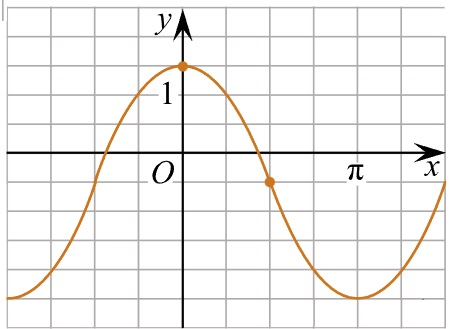
\includegraphics[align=t, width=\linewidth]{../pics/MECGERM6H3-1.jpg}
		\end{minipage}
		\item %тригон тг
		\begin{minipage}[t]{\bodywidth}
			На рисунке изображен график функции \(f(x) =a \tg x +b\). Найдите \(a\).
		\end{minipage}
		\hspace{0.02\linewidth}
		\begin{minipage}[t]{\picwidth}
			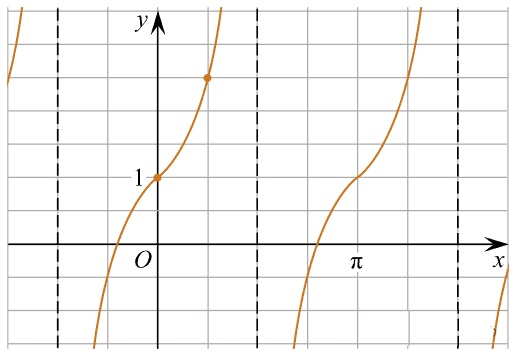
\includegraphics[align=t, width=\linewidth]{../pics/MECGERM6H3-2.jpg}
		\end{minipage}
		\item Найдите наименьшее значение функции \( y=4x-4 \ln(x+7)+6 \) на отрезке \( [-6,5;0] \). %3
		\item Найдите точку максимума функции \( y=\ln(x+5)^5-5x \) на отрезке. %12
		\item Найдите наибольшее значение функции \( y=12\cos x + 6\sqrt{3} x - 2 \sqrt{3} \pi + 6 \) на отрезке \( \left[ 0; \dfrac{ \pi }{ 2 } \right]  \).
	\end{listofex}
\end{homework}
%END_FOLD

%BEGIN_FOLD % ====>>_____ Занятие 7 _____<<====
\begin{class}[number=7]
	%\title{Подготовка к проверочной}
	\begin{listofex}
		\item Решите неравенства: %c192 a
		\begin{tasks}(2)
			\task \( \sqrt[ 7 ]{ 4x-9 } \ge 0 \) %1
			\task \( \sqrt[ 3 ]{ 5-2x } >0 \) %2
			\task \( \sqrt[ 7]{ 7x-8 } < 0 \) %13
			\task \( \sqrt[ 3 ]{ 9-x } \le -4 \) %16
			\task \( \sqrt[ 3 ]{ 3x^2-x-66 } > -4 \) %18
			\task \( \sqrt[ 9 ]{ 9x^2-12x+5 } \le 1 \) %19
			\task \( \sqrt[ 3 ]{ 3x-64 } < x-4 \) %c222 1
			\task \( \sqrt[ 3 ]{ x-2 } \ge \sqrt[ 3 ]{ x^3-3x+2 } \) %c222 3
		\end{tasks}
		\item %525392
		\begin{tasks}(1) 
			\task Решите уравнение: \( 2\log_{0,5}^2 (2\sin x) + 7 \log_{0,5} (2\sin x) + 3 = 0 \)
			\task Найдите все корни этого уравнения, принадлежащие отрезку: \( \left[ -\dfrac{3\pi}{2};0 \right] \)
		\end{tasks}
		
		\item Решите неравенства: %ctarie
		\begin{tasks}(2)
			\task \( |x^2-13| < 12 \)
			\task \( |2x^2-17| \le 15 \)
			%\task \( |2x^2-5x| \le 3 \)
			\task \( |x^2-15x| > 54 \)
			%\task \( |x^2-5x|<6 \)
			\task \( |x^2-20x|>96 \)
		\end{tasks}
	\end{listofex}
\end{class}
%END_FOLD

%BEGIN_FOLD % ====>>_ Занятие 8 _<<====
\begin{class}[number=8]
	\begin{listofex}
		\item Решите неравенства: %192 a 3 4 20 21 22 24 23 25 ДАЛЬШЕ БРАТЬ С С193
		\begin{tasks}(2)
			\task \( \sqrt[13]{5x+9} \le 0 \)
			\task \( \sqrt[5]{-11-4x} < 0 \)
			\task \( \sqrt[5]{8x-x^2-17} < -1 \)
			\task \( \sqrt[16]{4x-4x^2} \ge 1 \)
			\task \( \sqrt[]{x^2-5x+1} > 5 \)
			\task \( \sqrt[28]{8x-x^2-15} < 1 \)
			\task \( (x^2-24x)^{\tfrac{1}{4}} \le 3 \)
			\task \( (6x-x^2)^{\tfrac{1}{3}} \le 2 \)
		\end{tasks}
		\item Решите неравенства: %222 a 2 4 5 6 c193 25 26 a
		\begin{tasks}(1)
			\task \( \sqrt[]{x^2-144} \le 6 \)
			\task \( \sqrt{x^2-2x-15} < 3 \)
			\task \( \sqrt[3]{x^4-4x^3+7x^2+3x+1} \le x+1 \)
			%\task \( \sqrt[]{x^4-2x+6} \ge x \)
			%\task \( \sqrt[]{5x^4-28x^2+16} \ge x^2+4 \)
			%\task \( \sqrt[]{x^2-17x-29} \ge 3|x+2| \)
		\end{tasks}
	\end{listofex}
\end{class}
%END_FOLD

%BEGIN_FOLD % ====>>_ Консультация _<<====
\begin{consultation}
	\begin{listofex}
		%Первые 5 вписанные окружности
		\item Периметр треугольника равен \(12\), а радиус вписанной окружности равен \(1\). Найдите площадь этого треугольника.
		\item Площадь треугольника равна \(24\), а радиус вписанной окружности равен \(2\). Найдите периметр этого треугольника.
		\item Около окружности, радиус которой равен \(3\), описан пятиугольник, периметр которого равен \(20\). Найдите его площадь.
		\item Найдите радиус окружности, вписанной в правильный треугольник, высота которого равна \(6\).
		\item Радиус окружности, вписанной в правильный треугольник, равен \(6\). Найдите высоту этого треугольника.
		%Первые 3 описанные окружности
		\item Точки \(A, B, C,\) расположенные на окружности, делят ее на три дуги, градусные величины которых относятся как \(1 : 3 : 5\). Найдите больший угол треугольника \(ABC\). Ответ дайте в градусах.
		\item Угол \(A\) четырехугольника \(ABCD\), вписанного в окружность, равен \(58\degree\). Найдите угол \(C\) этого четырехугольника. Ответ дайте в градусах.
		\item Стороны четырехугольника \(ABCD \) \( AB, BC, CD, AD\) стягивают дуги описанной окружности, градусные величины которых равны соответственно \(95\) градусов, \(49\) градусов, \(71\) градусов, \(145\) градусов. Найдите угол \(B\) этого четырехугольника. Ответ дайте в градусах.
		%1,2,3,6 трапеции
		\item Основания равнобедренной трапеции равны \(51\) и \(65\). Боковые стороны равны \(25\). Найдите синус острого угла трапеции.
		\item Основания равнобедренной трапеции равны \(43\) и \(73\). Косинус острого угла трапеции равен \( \dfrac{5}{7} \).  Найдите боковую сторону.
		\item Большее основание равнобедренной трапеции равно \(34\). Боковая сторона равна \(14\). Синус острого угла равен \( \dfrac{2\sqrt{10}}{7} \). Найдите меньшее основание.
		\item Основания равнобедренной трапеции равны \(17\) и \(87\). Высота трапеции равна \(14\). Найдите тангенс острого угла.
		%\item %637451
		%\begin{tasks}(1)
		%	\task Решите уравнение \( \sin^3 x + \cos^3 x = \cos 2x \)
		%	\task Найдите все корни этого уравнения, принадлежащие отрезку: \( \left[ \dfrac{3\pi}{2}; 3 \pi \right] \)
		%\end{tasks}
		\item %638055
		\begin{tasks}(1)
			\task Решите уравнение \( 2\sin^2 x - (2+\sqrt{3})\cos \left( \dfrac{\pi}{2} - x \right) + \sqrt{3} = 0 \)
			\task Найдите все корни этого уравнения, принадлежащие отрезку: \( \left[ -\pi; \dfrac{\pi}{2} \right] \)
		\end{tasks}
	\end{listofex}
\end{exam}
%END_FOLD

%BEGIN_FOLD % ====>>_ Консультация _<<====
\begin{consultation}
	\begin{listofex}
		%Первые 5 вписанные окружности
		\item Периметр треугольника равен \(12\), а радиус вписанной окружности равен \(1\). Найдите площадь этого треугольника.
		\item Площадь треугольника равна \(24\), а радиус вписанной окружности равен \(2\). Найдите периметр этого треугольника.
		\item Около окружности, радиус которой равен \(3\), описан пятиугольник, периметр которого равен \(20\). Найдите его площадь.
		\item Найдите радиус окружности, вписанной в правильный треугольник, высота которого равна \(6\).
		\item Радиус окружности, вписанной в правильный треугольник, равен \(6\). Найдите высоту этого треугольника.
		%Первые 3 описанные окружности
		\item Точки \(A, B, C,\) расположенные на окружности, делят ее на три дуги, градусные величины которых относятся как \(1 : 3 : 5\). Найдите больший угол треугольника \(ABC\). Ответ дайте в градусах.
		\item Угол \(A\) четырехугольника \(ABCD\), вписанного в окружность, равен \(58\degree\). Найдите угол \(C\) этого четырехугольника. Ответ дайте в градусах.
		\item Стороны четырехугольника \(ABCD \) \( AB, BC, CD, AD\) стягивают дуги описанной окружности, градусные величины которых равны соответственно \(95\) градусов, \(49\) градусов, \(71\) градусов, \(145\) градусов. Найдите угол \(B\) этого четырехугольника. Ответ дайте в градусах.
		%1,2,3,6 трапеции
		\item Основания равнобедренной трапеции равны \(51\) и \(65\). Боковые стороны равны \(25\). Найдите синус острого угла трапеции.
		\item Основания равнобедренной трапеции равны \(43\) и \(73\). Косинус острого угла трапеции равен \( \dfrac{5}{7} \).  Найдите боковую сторону.
		\item Большее основание равнобедренной трапеции равно \(34\). Боковая сторона равна \(14\). Синус острого угла равен \( \dfrac{2\sqrt{10}}{7} \). Найдите меньшее основание.
		\item Основания равнобедренной трапеции равны \(17\) и \(87\). Высота трапеции равна \(14\). Найдите тангенс острого угла.
		%\item %637451
		%\begin{tasks}(1)
		%	\task Решите уравнение \( \sin^3 x + \cos^3 x = \cos 2x \)
		%	\task Найдите все корни этого уравнения, принадлежащие отрезку: \( \left[ \dfrac{3\pi}{2}; 3 \pi \right] \)
		%\end{tasks}
		\item %638055
		\begin{tasks}(1)
			\task Решите уравнение \( 2\sin^2 x - (2+\sqrt{3})\cos \left( \dfrac{\pi}{2} - x \right) + \sqrt{3} = 0 \)
			\task Найдите все корни этого уравнения, принадлежащие отрезку: \( \left[ -\pi; \dfrac{\pi}{2} \right] \)
		\end{tasks}
	\end{listofex}
\end{consultation}
%END_FOLD